% Asset ID: FA22TDistributionTikZ-002
% Source: Phase 1 lesson, paired versus independent samples section, Dr Frost paired/non-paired comparison slide and transcript
% Related lesson section: # 9.6 Paired versus independent samples
% Used placeholder: [VISUAL PLACEHOLDER: FA22TDistributionTikZ-002 | Source: Dr Frost paired/non-paired comparison slide + transcript | Insert from tikz/FA22TDistributionTikZ-002.tex | Purpose: Show why paired data becomes a one-sample test on differences.]
% Purpose: Show the structural difference between paired data and two independent samples.

\documentclass[tikz,border=8pt]{standalone}
\usepackage{amsmath}
\usepackage{xcolor}
\usetikzlibrary{arrows.meta,positioning,calc}
\definecolor{Canvas}{HTML}{FAF9F6}
\definecolor{Ivory}{HTML}{FFFFF0}
\definecolor{LineSoft}{HTML}{E5E5EA}
\definecolor{Gold}{HTML}{C5A059}
\definecolor{GoldBright}{HTML}{D4AF37}
\definecolor{PinkSoft}{HTML}{FBEFEF}
\definecolor{TextDark}{HTML}{2C2C2E}
\begin{document}
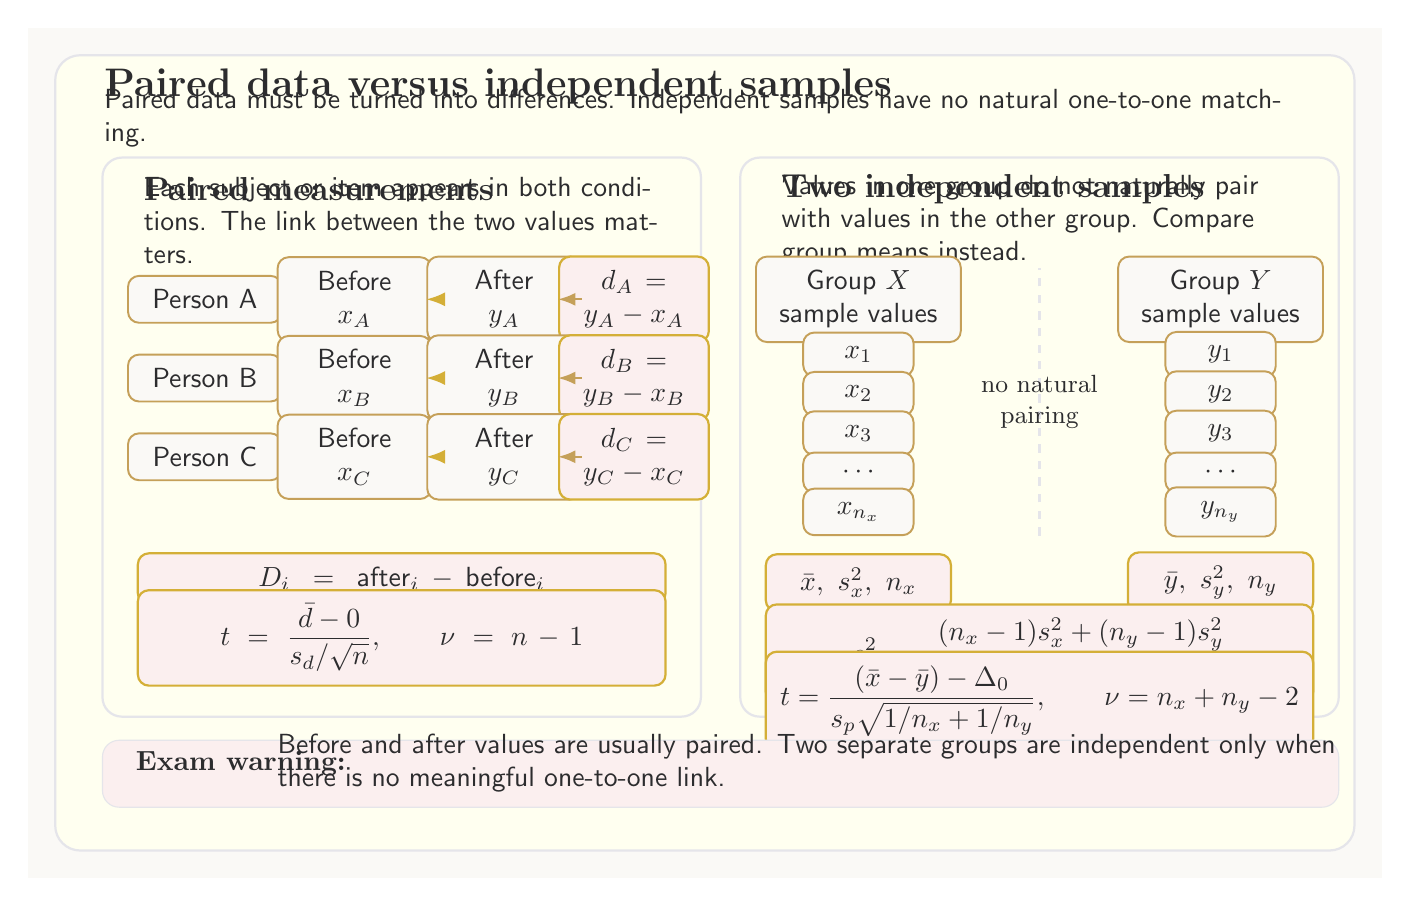
\begin{tikzpicture}[font=\sffamily,text=TextDark,>=Latex,box/.style={rounded corners=4pt,draw=Gold,fill=Canvas,line width=0.7pt,inner sep=5pt,align=center},diffbox/.style={rounded corners=4pt,draw=GoldBright,fill=PinkSoft,line width=0.8pt,inner sep=5pt,align=center}]
\fill[Canvas] (-0.8,-0.8) rectangle (16.4,10.0);
\draw[LineSoft,line width=0.8pt,rounded corners=9pt,fill=Ivory] (-0.45,-0.45) rectangle (16.05,9.65);
\node[anchor=west,font=\bfseries\Large] at (0.05,9.25){Paired data versus independent samples};
\node[anchor=west,text width=15.2cm] at (0.05,8.85){Paired data must be turned into differences. Independent samples have no natural one-to-one matching.};
\draw[rounded corners=7pt,draw=LineSoft,fill=Ivory,line width=0.8pt] (0.15,1.25) rectangle (7.75,8.35);
\draw[rounded corners=7pt,draw=LineSoft,fill=Ivory,line width=0.8pt] (8.25,1.25) rectangle (15.85,8.35);
\node[anchor=west,font=\bfseries\large] at (0.55,7.95){Paired measurements};
\node[anchor=west,font=\bfseries\large] at (8.65,7.95){Two independent samples};
\node[anchor=west,text width=6.8cm] at (0.55,7.55){Each subject or item appears in both conditions. The link between the two values matters.};
\node[anchor=west,text width=6.8cm] at (8.65,7.55){Values in one group do not naturally pair with values in the other group. Compare group means instead.};
\foreach \p/\y in {A/6.55,B/5.55,C/4.55}{
\node[box,text width=1.6cm] (p\p) at (1.45,\y){Person \p};
\node[box,text width=1.6cm] (b\p) at (3.35,\y){Before\\\(x_\p\)};
\node[box,text width=1.6cm] (a\p) at (5.25,\y){After\\\(y_\p\)};
\node[diffbox,text width=1.55cm] (d\p) at (6.9,\y){\(d_\p=y_\p-x_\p\)};
\draw[-{Latex[length=2.4mm]},draw=GoldBright,line width=0.9pt] (b\p) -- (a\p);
\draw[-{Latex[length=2.2mm]},draw=Gold,line width=0.8pt] (a\p) -- (d\p);
}
\node[diffbox,text width=6.35cm] at (3.95,3.0){\(\displaystyle D_i=\text{after}_i-\text{before}_i\)};
\node[diffbox,text width=6.35cm] at (3.95,2.25){\(\displaystyle t=\frac{\bar d-0}{s_d/\sqrt n},\qquad \nu=n-1\)};
\node[box,text width=2.25cm] at (9.75,6.55){Group \(X\)\\sample values};
\node[box,text width=2.25cm] at (14.35,6.55){Group \(Y\)\\sample values};
\foreach \y/\lab in {5.85/{\(x_1\)},5.35/{\(x_2\)},4.85/{\(x_3\)},4.35/{\(\cdots\)},3.85/{\(x_{n_x}\)}}{\node[box,text width=1.05cm,minimum height=0.32cm] at (9.75,\y){\lab};}
\foreach \y/\lab in {5.85/{\(y_1\)},5.35/{\(y_2\)},4.85/{\(y_3\)},4.35/{\(\cdots\)},3.85/{\(y_{n_y}\)}}{\node[box,text width=1.05cm,minimum height=0.32cm] at (14.35,\y){\lab};}
\draw[LineSoft,line width=1.2pt,dashed] (12.05,3.55) -- (12.05,6.95);
\node[align=center,font=\small,text width=2.1cm] at (12.05,5.25){no natural\\pairing};
\node[diffbox,text width=2.0cm] at (9.75,2.95){\(\bar x,\ s_x^2,\ n_x\)};
\node[diffbox,text width=2.0cm] at (14.35,2.95){\(\bar y,\ s_y^2,\ n_y\)};
\node[diffbox,text width=6.6cm] at (12.05,2.05){\(\displaystyle s_p^2=\frac{(n_x-1)s_x^2+(n_y-1)s_y^2}{n_x+n_y-2}\)};
\node[diffbox,text width=6.6cm] at (12.05,1.45){\(\displaystyle t=\frac{(\bar x-\bar y)-\Delta_0}{s_p\sqrt{1/n_x+1/n_y}},\qquad \nu=n_x+n_y-2\)};
\draw[LineSoft,rounded corners=6pt,fill=PinkSoft] (0.15,0.1) rectangle (15.85,0.95);
\node[anchor=west,font=\bfseries] at (0.45,0.66){Exam warning:};
\node[anchor=west,text width=13.6cm] at (2.25,0.66){Before and after values are usually paired. Two separate groups are independent only when there is no meaningful one-to-one link.};
\end{tikzpicture}
\end{document}
